% !TeX root = ../praktikum.tex
% !TeX encoding = UTF-8
% !Tex spellcheck = de_DE

Im folgendem Abschnitt wurden die Messungen des vorigen Versuchsteils im Wesentlichen wiederholt, mit dem Unterschied, dass anstatt eines Gleichstroms ein Wechselstrom angelegt %TODO: Spannung oder SStrom?! 
 %mit $U_{RMS}=\unit[1]{V}$ angelegt wurde und ein \unit[9,95]{$M\Omega$} Widerstand in Reihe geschaltet wurde. 
 Um einen Wechselstrom erzeugen zu können, wurden sogenannte Lock-in Verstärker genutzt. Ein Lock-in Verstärker enthält einen Funktionsgenerator, welcher anhand einer einstellbaren Frequenz eine sinusförmige Wechselspannung mit $U_{RMS}=\unit[1]{V}$ ausgibt. Um den Strom unabhängig von dem Widerstand des Hall-Streifens zu halten, musste ein hinreichend großer Widerstand in Reihe geschaltet werden. Da der Eigenwiderstand des Hall-Streifens bei einigen Megaohm lag, wurde ein  \unit[9,95]{$M\Omega$} Widerstand verwendet. So kann in guter Näherung angenommen werden, dass der Strom allein durch den zusätzlich angelegten Vorwiderstand zu $I=\nicefrac{U}{R}=\nicefrac{\unit[1]{V}}{\unit[9,95]{M\Omega}}=\unit[0,995]{\mu A}$ bestimmt wurde. 
 Bei der Durchführung der Wechselstrommessung fiel auf, dass die Plateaus im Graphen der Hallspannung %TODO: Hallwiderstand?
 deutlich ausgeprägter ausfielen, als für die Gleichstrommessung. Analog dazu waren hier schmalere Peaks in der Shubnikov-de Haas-Oszillation zu erkennen.  
 Erneut konnte die Formel~\eqref{eq:u2rho} genutzt werden, um den Widerstand aus dem Spannungsabfall zu erhalten. %TODO: Hallwiderstand?

\begin{figure}[h]
	\centering
	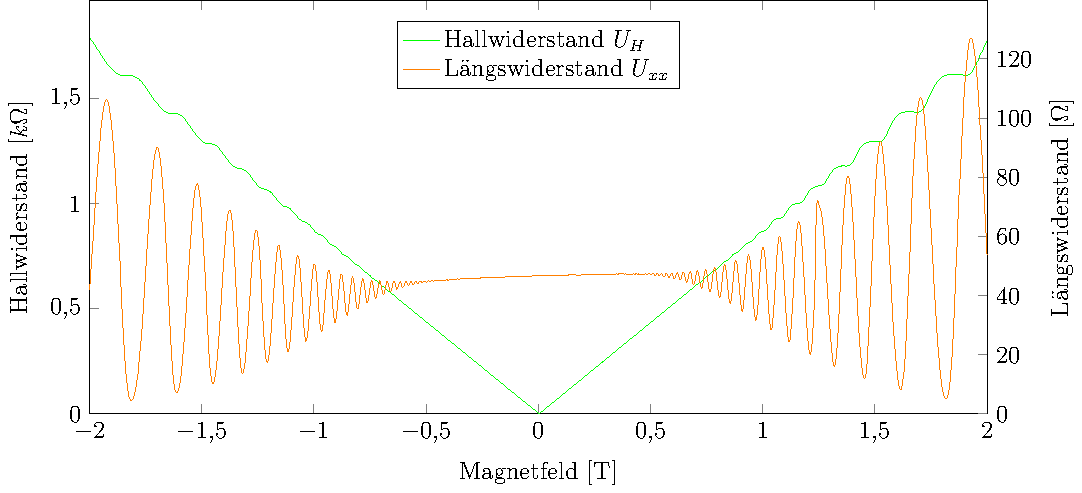
\includegraphics{graphs/ac/pm2T_range.pdf}
	\caption[Höher aufgelöste Gleichstrommessung in Magnetfeldteilbereich]{
		Hall-Widerstand und Shubnikov-de Haas Oszillationen eines mit Gleichstrom durchflossenen 2DES.
	}
	\label{fig:2T_range_ac}
\end{figure}


\begin{figure}[h]
	\centering
	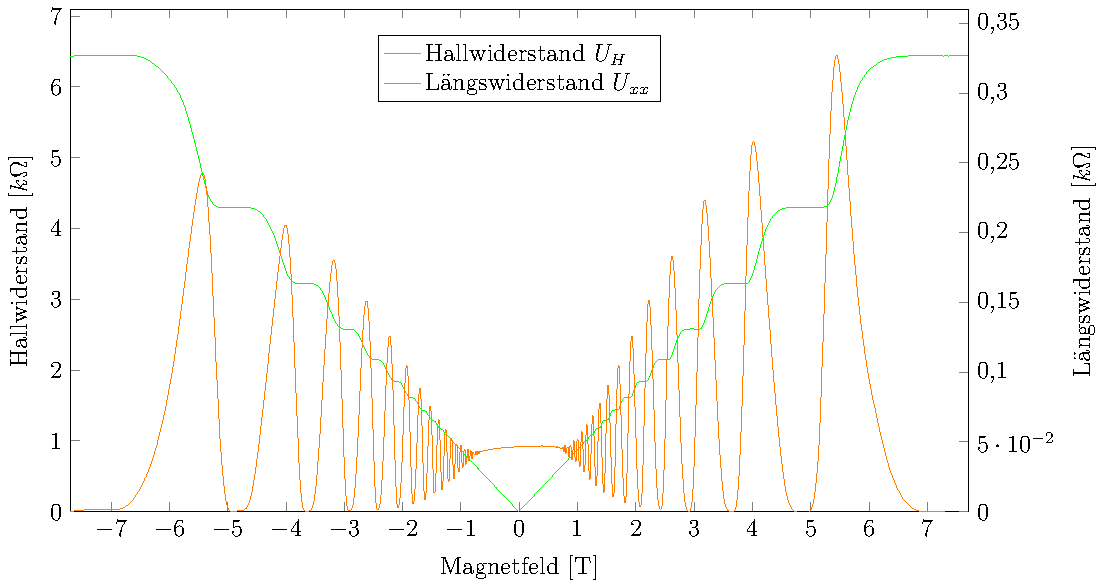
\includegraphics{graphs/ac/full_range.pdf}
	\caption[Wechselstrommessung im maximalen Magnetfeldbereich]{
		Hall-Widerstand und Shubnikov-de Haas Oszillationen eines mit Wechselstrom durchflossenen 2DES.
	}
	\label{fig:full_range_ac}
\end{figure}


